\section{Индексация}

Задачей, не связанной напрямую с полнотекстовым поиском и решением для его осуществления, является индексация, а именно транспорт данных из первичного источника в поисковые индексы. Так как индексы являются специальной структурой данных, они не обязаны давать доступ к первичным данным, перед тем, как те были проанализированы, приведены к набору термов и в таком виде сохранены. Кроме того, хранение данных в системах, которые не гарантируют линеаризуемость чревато потерями данных, что недопустимо для многих реальных приложений.

Однако если есть отдельно система надежного хранения данных и отдельно полнотекстовые индексы, необходимо, чтобы, во-первых, данные, попадая в первичный источник, попадали также в индексы. И кроме того, при сбое в системе хранения индексов, необходимо, чтобы данные синхронизировались и за конечное время оказывалось, что все документы, находящиеся в первичном хранилище, проиндексированы и доступны для поиска.

\subsection{Индексатор}

Индексатор~--- программа, внешняя по отношению к первичному хранилищу данных и поисковым индексам, которая выполняет функции описанные выше, то есть синхронизирует данные между указанными двумя. Существует два способа организации процесса индексации, в первом случае, работа индексатора организована в бесконечном цикле, на каждой итерации которого происходит работа, во втором случае создается система, основанная на событиях и их обработке. Однако во втором случае работа с ошибками индексации становится сложнее, так как необходимо генерировать отдельные события. Также необходимо организовать первичный перенос данных, уже находящихся в первичном источнике на момент начала работы индексатора.

\subsubsection{Цикл индексации}

В общем случае итерация цикла индексации организована следующим образом:

\begin{enumerate}
	\item Прочитать набор документов из первичного источника
	\item Преобразовать исходные документы
	\item Отправить запрос на индексацию преобразованных документов
	\item Приостановить выполнение на некоторое время
\end{enumerate}

Шаг преобразования необходим для общности. Например, он может включать формирования запроса не на добавление документа в индекс, а на изменение существующего. Кроме того, не всегда есть потребность во всех данных, возможно в индекс будет отправлять какой-то срез. Также возможны ситуации, когда шаг преобразования не востребован и данные, прочитанные из первичного источника данных, сразу же отправляются в индексы, что является вполне корректным сценарием поведения.

\subsubsection{Состояние}

Индексатор не может существовать сам по себе, у него должна присутствовать внешняя часть, которая будет работать независимо от работы самого индексатора. Она будет содержать информацию о текущем прогрессе, то есть о том, какие документы уже прочитаны и проиндексированы, а какие документы еще подлежат обработке. Данная внешняя часть может быть реализована как файл в файловой системе, документ в базе данных, область памяти программы, запущенной независимо и любым другим способом, который обеспечивает независимость данного состояния от процесса индексации.

Наличие состояния продиктовано необходимость допустить возможность завершения программы индексатора, как в силу всевозможных ошибок и отказов, так и в силу намеренных действий. Если состояние будет целиком частью индексатора, то при подобном перезапуске не будет доступна информация, какие документы уже были проиндексированы, а какие еще только следует прочитать из первичного источника. Таким образом у индексатора появляется внешний интерфейс, который диктует ему входные данные и сохраняет прогресс.  Подобный инструмент является первым шагом к достижению надежности системы индексации.

\subsubsection{Модульность и унификация}

Так как задач по индексации существует большое количество, то возникает необходимость в ускорении разработки за счет унифицирования узлов и переиспользования уже использованной логики. Например, одни и те же данные по способу организации могут быть проиндексированы одним и тем же индексатором, по-разному сконфигурированным. Однако редко бывает так, что данные полностью совпадают по формату и логике обработке. Из архитектуры рабочего цикла индексатора следует наличие трех независимых компонент, на которые этот индексатор можно разделить~--- компонента для чтения, компонента для преобразования документов и компонента для составления запроса на индексацию для конкретных документов. Используя такую модульность и возможность независимо конфигурировать разные компоненты, мы получаем гораздо больший простор для переиспользования логики. Например, есть модуль для чтения документов из базы данных, конфигурируя его именем коллекции, из которой брать данные, и типом данных, можно менять приложения получающего индексатора, причем радикально. 

\subsubsection{Отказоусточивость и надежность}

Держа в уме тот факт, что существует большое количество ситуаций, в которых программное обеспечение выходит из строя, нельзя не обращать внимание на корректную обработку подобных случаев. Самым простейшим способом реагировать на ситуации в случае отказов можно автоматически перезапуская процесс индексации, например средствами операционной системы или специализированных программ. Однако это, во-первых, не спасает от отказов на уровне вычислительного узла, когда операционная система и все программы прикладного уровня перестают функционировать, во-вторых, не обеспечивает достаточной информативностью в случае ошибки, которая приводит к постоянному перезапуску индексатора.

Ввиду вышесказанного возникает необходимость создания специализированной распределенной системы запуска индексаторов, которая позволила бы выполнить требования по отказоустойчивости и надежности системы в целом. Как и в любой распределенной системе от нее требуется решения определенного класса задач, в том числе в данном случае, наличие линеаризуемости и устойчивости к разделению сети.

\subsubsection{Существующие решения}

Индексаторы, будучи очень сильно завязанными на конкретные типы данных и бизнес-процессы, чаще всего оставляются на откуп разработчиком конкретного продуктового решения, однако существуют некоторые универсальные программы с готовым набором конфигурируемых модулей, которые позволяют ускорить разработку и облегчить введение полнотекстового поиска в эксплуатацию.

Одним из самых известных решений является Logstash. Он в точности реализует схему, указанную выше, обладая тремя независимыми конфигурируемыми компонентами. Любую из них чаще всего можно реализовать с помощью настройки готовых модулей. Этот продукт активно продвигается создателями Elasticsearch, он действительно позволяет просто и быстро настроить даже не очень простой процесс непрерывной индексации данных их произвольного источника в полнотекстовый индекс. Главным его недостатком является то, что он не реализует логику, связанную с решением задачи распределения процесса индексации на несколько компьютеров. Logstash представляет собой программу, которая работает, будучи вручную запущена в операционной системе. Это четко следует принципу разделения ответственности между программами, но делает выбор в стороны данного решения невозможным.

Также существует множество решений, предложенных сообществом, для решения задачи индексации, но нет сопоставимого Logstash по расширяемости и гибкости, и тем более нет такого, который был, согласуясь с платформой разработки программного обеспечения, используемой в компании, заинтересованной в решении рассматриваемой задачи, предоставлял одновременно как богатые возможности по конфигурации и настройке, так и решение задачи распределения процесса индексации на множество вычислительных узлов.

\subsubsection{Требования к решению}

После безуспешной попытки найти решение среди существующих на данный момент, было очевидно, что необходимо создать свой продукт. Для того, чтобы определить, что необходимо проделать, было выдвинуто несколько требований, которым должно удовлетворять решение, чтобы можно быть считать его готовым к использованию в реальном окружении. Требования включали, но не ограничивались следующими пунктами:

\begin{itemize}
	\item Модульность
	\item Наличие готовых компонентов
	\item Расширяемость
	\item Гибкость, высокая степень конфигурируемости
	\item Надежность, отказоустойчивость
\end{itemize}

В результате анализа возможного решения было выделено две независимые задачи, которые в сумме составили бы систему, удовлетворяющую вышеизложенным требованиям. Первая компонента, плагин, представляет собой некоторый скелет логики по индексации, хорошо расширяемый за счет модулей, в том числе некоторых готовых. Плагины при этом имеют некоторый внешний интерфейс, унифицирующий работу с состоянием, запуск и остановку. Вторая компонента представляет собой распределенную систему для запуска плагинов, доставляя до них существующее состояние, сохраняющее прогресс и отслеживающая ошибки и отказы, происходящие с отдельно взятыми экземплярами.

\subsection{Плагины}

\subsubsection{Компоненты}

Плагин конфигурируется следующими компонентами, каждая из которых имеет свою зону ответственности и не зависит напрямую от других, и в частности может быть отдельно сконфигурирована:

\begin{itemize}
	\item Reader
	\item Primary Key Extractor
	\item Document Factory
	\item Merger
\end{itemize}

\paragraph{Reader}

Данная компонента отвечает за чтение данных из первичного источника, как то например из базы данных. В рамках платформы, предоставляемой конечному пользователю системы, в частности, предлагается готовая вариация, читающая данные из локально разработанной системы хранения информации. Так как чтение напрямую связано с внутренним состоянием индексатора, то именно в этой части сконцентрирована работа с ним. Кроме интерфейса для чтения, Reader дает возможность установить состояние в данное или считать текущее, чтобы отслеживать и контролировать осуществляемый прогресс. Заметим также, что данный интерфейс обеспечивает чтение \textbf{входных данных}, назначение которых будет определено позднее.

\paragraph{Primary Key Extractor}

Для того, чтобы однозначно определить, к какому документу относится прочитанная часть входных данных, необходим некоторый уникальный идентификатор. Данный интерфейс определяет логику по извлечению подобного индексатора, предоставляя возможность по входным данным получить строку, уникальную для каждого документа в итоговом индексе, доступном для поиска.

\paragraph{Document Factory}

После того, как для входных данных был определен уникальный идентификатор, по нему происходит поиск в индексе, на случай, если такой документ уже существует и доступен для поиска. Если документа не обнаружилось, то необходимо инициализировать его из входных данных. Логика по подобной инициализации и заключена в данном интерфейсе.

\paragraph{Merger}

Если документ уже был найден в индексе, то входные данные заключают в себе изменения, которые необходимо применить к уже существующему документу. Логика по тому, как документу и входных данным сопоставить документ, отражающий внесенные правки и заключается в данной компоненте. 

\subsubsection{Принцип работы}

Плагин заключает в себе два логических потока выполнения, первый занимается непрерывным чтением данных из источника и добавлением их в очередь, второй осуществляет функцию индексатора, преобразуя и индексируя прочитанные в первом потоке данные.

Логика выполнения потока чтения грубо может быть представлена в виде следующего алгоритма

\begin{enumerate}
	\item Прочитать объект из источника
	\item Добавить в формирующееся множество исходных данных
	\item Если размер текущего множества меньше фиксированной величины, вернуться на шаг 1
	\item Иначе, зафиксировать текущее состояние Reader'а и добавить в очередь на индексацию пару из текущего состояния и множества исходных данных
	\item Обнулить множество исходных данных и перейти на шаг 1
\end{enumerate}

Размер множества исходных данных ограничивается некоторой величиной, которая конфигурируется отдельно для каждого плагина в системе, ровно, как и максимальный размер очереди, при превышении которого поток чтения будет приостановлен до момента, когда освободится место. Данная системы была введена для ускорения процесса индексации, так как процесс чтения является достаточно времязатратным и при этом независимым.

Логика потока выполнения индексации в свою очередь может быть описана следующим образом

\begin{enumerate}
	\item Взять множество исходных данных и состояние из очереди
	\item Получить идентификатор каждого объекта исходных данных
	\item Получить из индекса документы для каждого идентификатора
	\item Пройтись по всем объектам исходных данных в порядке их чтения и либо создать новый документ, либо применить изменение к уже существующему
	\item Проиндексировать получившиеся документы
	\item Для всех объектов исходных данных, принадлежащих документам, которые не проиндексировались в силу какой-либо ошибки, повторить шаги начиная с 3
	\item Считать, что были проиндексированы документы до состояния, взятого ранее из очереди
\end{enumerate}

Кроме того, существует ограничение на количество попыток проиндексировать документы, которые вызывают ошибку, чтобы не возникло опасности возникновения бесконечного цикла без какого-либо прогресса. Функции взаимодействия с документами и объектами исходных данных реализованны с помощью вышеописанных компонент.

За счет того, что состояние сохраняется после того, как все документы, прочитанные до перехода в это состояние, были успешно проиндексированы, мы можем сказать, что невозможно получить извне состояние более новое, чем то, которое соответствует по меньшей мере не более новым данным, чем были на самом деле проиндексированы.

\subsection{Система запуска плагинов}

Распределенная система запуска плагинов также разбивается на несколько функциональных компонент, каждая из которых занимает свою роль в итоговой картине. Три роли охватывают поверхностно картину системы со стороны, а именно

\begin{itemize}
	\item Master~--- часть, которая отвечает за хранение метаданных о существующих плагинах, распределение плагинов по существующим вычислительным мощностям, обработку и хранение ошибок
	\item Host~--- часть, напрямую взаимодействующая с плагинами. Хост получает информацию от мастера, какие плагины необходимо запустить, стартует их и следит за последующим выполнением
	\item Monitoring~--- интерфейс для администратора данной системы, который позволяет получить доступ к созданию новых плагинов, конфигурированию существующих и анализу произошедших событий в кластере
\end{itemize}

Кроме перечисленных компонентов, для корректного функционирования системы необходимо также несколько внешних систем, как то сервис распределенных блокировок и внешняя система хранения данных для исходного кода плагинов и система хранения данных для состояния мастера. Общая схема системы в целом выглядит следующим образом:

\begin{figure}[h]
	\centering
	\caption{\textbf{Схема кластера системы запуска индексаторов}}
	
	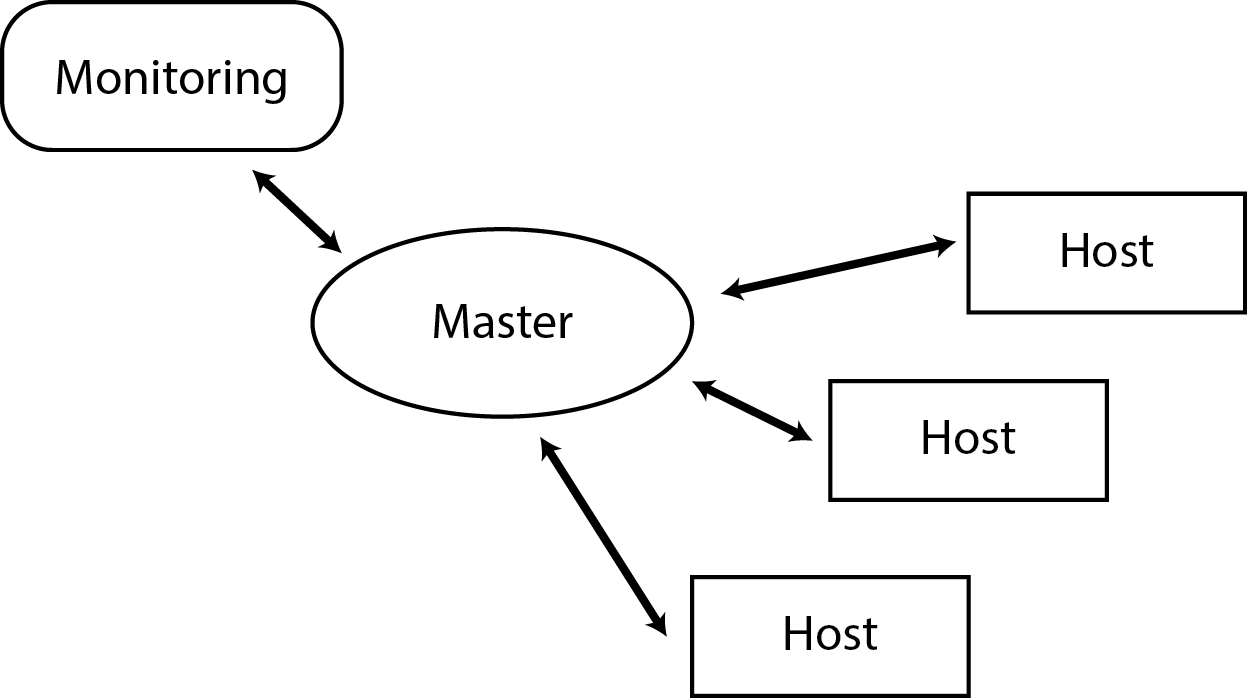
\includegraphics{0-basic-scheme}
\end{figure}

Далее в отдельности рассмотрим каждую компоненту системы

\subsubsection{Мастер}

Мастер представляет собой мета-состояние кластера и содержит в себе информацию о каждом существующем плагине, его состоянии, конфигурации, случившихся ошибках и поддерживает внешний интерфейс, доступный конечному пользователю, для изменения этого состояния. Для того, чтобы мастер не являлся единой точкой отказа в системе, одновременно существует несколько запущенных мастеров. С помощью внешнего механизма распределенных блокировок мастера выбирают одного, который единственный имеет после этого возможность изменять состояние.

Кроме того, перед тем, как изменение будет применено к состоянию, оно записывается в лог операций. Каждая операция надежно сохраняется в хранилище, для которого доказано свойство консистентности.

\begin{figure}[h]
	\centering
	\caption{\textbf{Схема устройства мастера (кластера мастеров)}}
	
	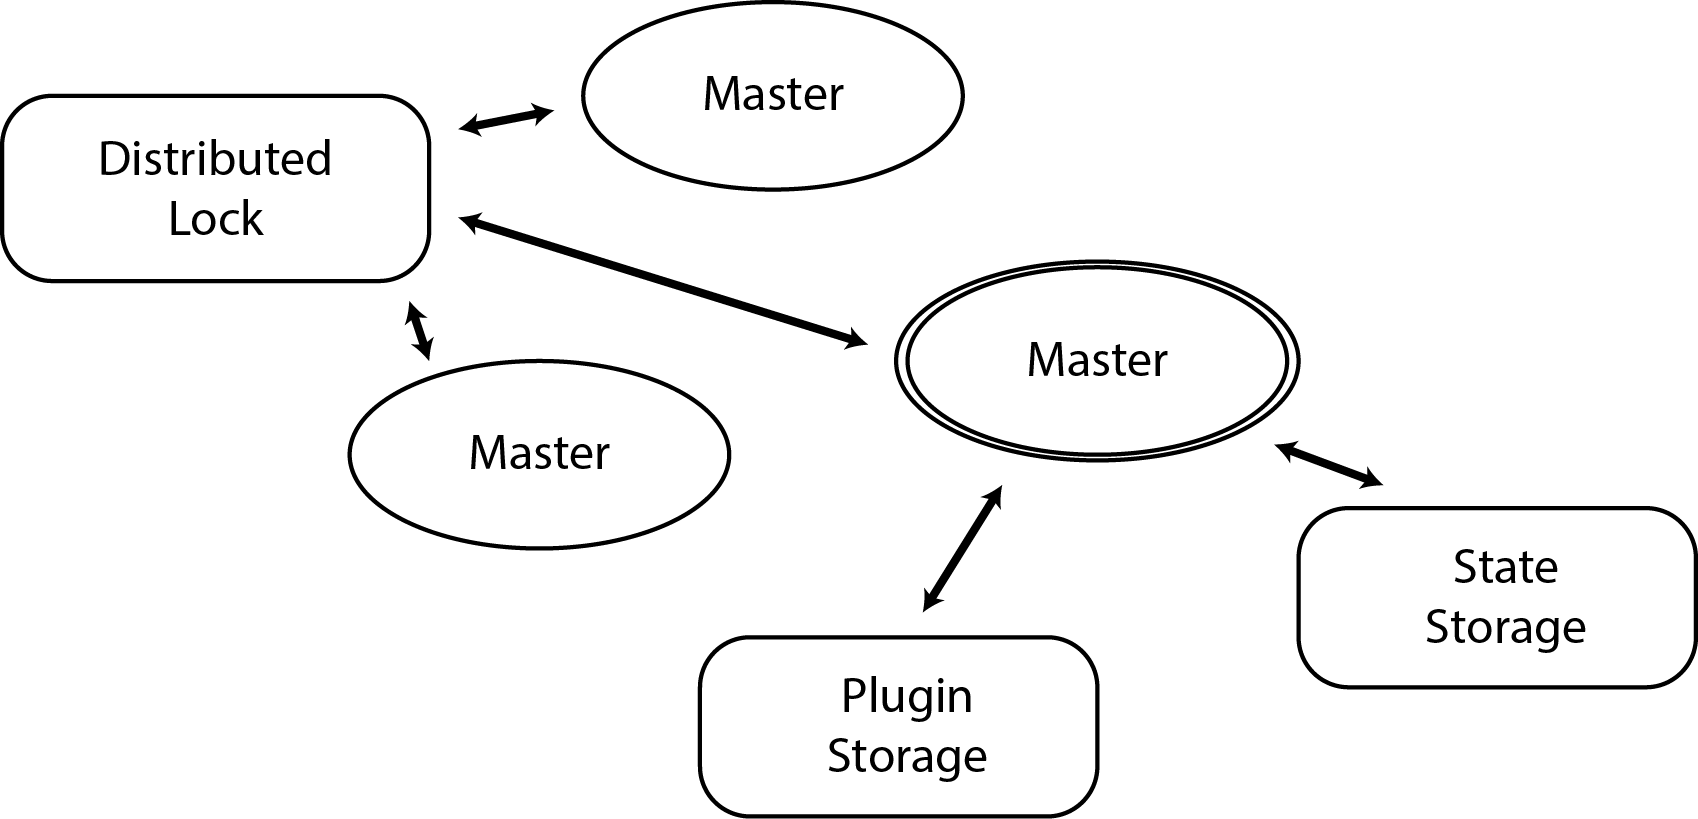
\includegraphics{1-master-scheme}
\end{figure}

Иногда может произойти так, что мастер, который в данный момент держит единоличное право на оперирование с состоянием, выйдет из строя. Тогда с помощью все того же внешнего механизма распределенной блокировки выбирается новый мастер, который занимает место вышедшего из строя. Таким образом, даже при множественном отказе мастера, покуда существует хотя бы один, успешно функционирующий и покуда функционирует система распределенных блокировок, рассматриваемая система будет функционировать.

Для оперирования плагинами в мастере есть механизм аренд, который выдает конкретному хосту уникальное в данный момент право на владение плагином, то есть на его запуск. Для поддержания аренд хосты периодически отсылают мастеру сообщения со своим текущим состоянием. На основании этих сообщений возможны изменения решений о выдаче аренд. Также из сообщений от хоста берется некоторая информация для сохранения в текущее состояние мастера. Если на протяжении продолжительного времени от хоста не приходит сообщение, то мастер считает этот хост вышедшим из строя и назначает плагины, назначенные на этот хост, на другие хосты.

\subsubsection{Хост}

Задача хоста~--- периодически информировать мастера о своем состоянии, получать от него список индексаторов, которые еще не были запущены и запускать их. Кроме того, хост также отправляет мастеру информацию о том, какие плагины запущенны в данный момент, их состояние и различные метрики, а также ошибки, которые произошли в процессе работы. Если хост получает информацию о том, что у него не запущен плагин, который назначен на него в состоянии мастера, он сначала скачивает исполняемый код из выделенного хранилища, внешнего по отношению к рассматриваемой системе, затем запускает цикл исполнения скачанного кода, перезапуская плагин по мере надобности, если ошибка привела к его немедленной остановке.

Немаловажной задачей хоста является запись метрик во внешнее хранилище для мониторинга и построения аналитики. Для расследования аномальных ситуаций администратором необходимо понимать текущее состояние ресурсов, выделенных операционной системой на задачу хоста, а также иметь перед глазами историю изменения потребления данных ресурсов на протяжении некоторого времени, для осуществления правильного в текущий момент действия, направленного на стабилизацию ситуации и нормализации работы системы.

\subsubsection{Мониторинг}

Одним из важных компонентов системы является мониторинг, который содержит информацию о текущем состоянии кластера и позволяет через него осуществлять манипуляции с плагинами, их конфигурациями и состояниями. Мониторинг по сути является промежуточным пунктом между администратором, который контролирует работоспособность системы и мастером, управляющим плагинами в автоматическом режиме. 

\clearpage
